\section{Business use cases}
\label{sec:business-use cases}
	
	This section presents the core business use cases that have been identified in discussions with the SU team members. These use cases have been structured in the light of the new asset lifecycle process, and not the current one, even though they are heavily inspired by the current asset lifecycle process. Section \ref{sec:business-architecture} will present the designs of the current and the new asset lifecycle processes illustrating differences and commonalities. The designed processed are a derived from the use case descriptions following below. 
	
	\subsection{UC1: Evolution: Register request for content change}
	\label{sec:uc1}
	
	\textbf{Trigger:} A request for content change is received in the functional mailbox
	
	\textbf{Success guarantee:} A complete and clear change request case is created and scheduled for approval.
	
	\textbf{Main success scenario:}
	
	\begin{enumerate}
		\item The client requests a change of one or multiple concepts in an asset
		\item The request manager creates a new change request case and acknowledges the client
		\item The asset manager analyses the request (in terms of business needs and in term of data management implications) and summarises the case
		\item Request manager informs the client of the case summary
		\item The request manager proposes the case for discussion in the next meeting of the team steering committee		
	\end{enumerate}
	\textbf{Extensions:}
	\begin{enumerate}
		\item [4a] The request is incomplete or unclear:
		\begin{enumerate}
			\item [4a1] The asset manager formulates the information needs			
			\item [4a2] The request manager collects the needed details and clarifications from the client
			\item [4a3] Return to step 3 
		\end{enumerate}
		\item [4b] The request is complex and needs deeper conceptual analysis and modelling/design:
		\begin{enumerate}
			\item [4b1] The asset manager presents the case to the knowledge modelling expert 
			\item [4b2] The knowledge modelling expert analyses the case and proposes a solution
			\item [4b3] Return to step 3			
		\end{enumerate}
	\end{enumerate}
	
	
	\subsection{UC2: Evolution: Register request for content change}
	\label{sec:uc2}
	
	\textbf{Trigger:} A team steering committee meeting takes place 
	
	\textbf{Preconditions:} A case is in the meeting agenda 
	
	\textbf{Success guarantee:} The case is rejected or approved for implementation
	
	\textbf{Main success scenario:}
	
	\begin{enumerate}
		\item Any time between the case is proposed for discussion and the meeting, committee members may assess the open cases and add business, technical or implementation related comments. 
		\item During the meeting, the asset manager presents the case.
		\item The steering committee members discuss, comment the case
		\item The steering committee approves the case for implementation
		\item Asset manager schedules the case for implementation		
	\end{enumerate}
	\textbf{Extensions:}
	\begin{enumerate}
		\item [4a] The case is rejected:
		\begin{enumerate}
			\item [4a1] The steering committee reject the case along with a justification
			\item [4a2] The request manager informs the client and provides recommendations			
		\end{enumerate}
		\item [4b] The case needs additional input:
		\begin{enumerate}
			\item [4b1]  The steering committee reject the case along with a request for action, information or agreement to an alternative proposal
			\item [4b2] The request manager informs the user and requests additional actions, information or agreement to an alternative proposal
			\item [4b3] The request manager register request for content change (UC1)
		\end{enumerate}
	\end{enumerate}

	\subsection{UC3: Implementation: Implement request for content change}
	\label{sec:uc3}
	
	\textbf{Trigger:} A case is scheduled for implementation
	
	\textbf{Preconditions:} The case is approved for implementation
	
	\textbf{Success guarantee:} The case is implemented and validated, while the data are exported and stored in the common repository
	
	\textbf{Main success scenario:}
	
	\begin{enumerate}
		\item The request manager schedules a case for implementation
		\item Data authoring officer reads the case and executes the content authoring accordingly
		\item Data authoring officer automatically or assisted by the data processing officer
		\begin{enumerate}
			\item exports the asset from the authoring tool and 
			\item runs the SHACL validation for conceptual and structural issues and
			\item runs the difference calculation between exported content and the previous release export and
			\item runs the fingerprint calculation for the exported content
			\item the data and reports are stored in the common repository 
		\end{enumerate}		
		\item Data authoring officer checks 
		\begin{enumerate}
			\item (verification) that the diff report calculated between the previous release export corresponds to the implemented change request\footnote{This is to validate that the export reflects change request case for the change request ticket, keeping the editors on the safe side. If all is good, then this is the final diff.}.
			\item (validation) that no structural anomalies are present in the fingerprint and validation reports
		\end{enumerate}		 
		\item Repeat steps 1 - 4 until all cases are implemented for the asset
		\item Data authoring officer informs the quality assurance officer of the successful implementation of all cases.		
	\end{enumerate}
	
	\textbf{Extensions:}
	\begin{enumerate}
		\item [2a] Translations are necessary:
		\begin{enumerate}
			\item [2a1] Additionally, data authoring officer manages the necessary translations and proof-reading (process described elsewhere: export selected data for translators, send to the translation unit,  import updated data containing the translations, validate and proofread the translations)			
		\end{enumerate}
		\item [4a] Implementation or data is invalid:
		\begin{enumerate}
			\item [4a1] Data authoring officer collects and documents all the issues 
			\item [4a2] Return to step 2			
		\end{enumerate}
	\end{enumerate}
	
	\subsection{UC4: Validation: Validate the request for change}
	\label{sec:uc4}
	
	\textbf{Trigger:} An implementation is scheduled for validation (data available in SRC-AP format along the assessment reports)
	
	\textbf{Preconditions:} All the cases are implemented for an asset and no further updates are foreseen
	
	\textbf{Success guarantee:} The data are validated by a second pair of eyes and marked as fit for publication
	
	\textbf{Main success scenario:} 
	
	\begin{enumerate}
		\item Data authoring officer provides the data and validation reports in the common repository 
		\item Quality assurance office verifies that the diff report corresponds to case requirements
		\item Quality assurance office checks the fingerprint and validation reports for semantic or structural anomalies. 
		\item Quality assurance office accepts the implementation and the data and informs the asset manager
		\item Asset manager marks the asset as fit for publication.
		
	\end{enumerate}
	
	\textbf{Extensions:}
	
	\begin{enumerate}
		\item [4a] Data quality issues are detected:
		\begin{enumerate}
			\item [4a1] The quality assurance officer identifies  and documents issues in the validation and fingerprint reports and informs the data authoring officer what the issues are and eventually explains how to fix them.
			\item [4a2] Data authoring officer implements the request for change (UC3)			
		\end{enumerate}
		\item [4b] Implementation issues are detected:
		\begin{enumerate}
			\item [4b1] The quality assurance officer identifies and documents issues in the diff report and informs the data authoring officer what the issues are and eventually explains how to fix them.
			\item [4b2] Data authoring officer implements the request for change (UC3)			
		\end{enumerate}
	\end{enumerate}


	\subsection{UC5: Release: Prepare the publication content}
	\label{sec:uc5}
	\textbf{Trigger:} Asset release is requested
	
	\textbf{Preconditions:} 
	\begin{itemize}
		\item The data is conceptually and formally validated (SRC-AP) and its content is fit to be published
		\item Code freeze is declared, no more changes are foreseen
	\end{itemize}
	
	\textbf{Success guarantee:} The data are available in standard (and where requested additional) forms and formats.
	
	\textbf{Main success scenario:}
	
	\begin{enumerate}
		\item Asset manager requests a release
		\item Data processing officer start the transformation processes from SRC-AP form into 
		\begin{enumerate}
			\item Target forms: SKOS-AP-EU/Act/Core
			\item Target formats: RDF/XML, Turtle, JSON-LD
		\end{enumerate}		
		\item Data processing officer runs the fingerprinting and SHACL validation for structural issues and confirms the transformation went well\footnote{This process is automatic and has the purpose of ensuring the transformation process passed correctly, keeping the data processing officers on the safe side.}.
		\item Data processing officer start the transformation processes from SRC-AP/SKOS-AP-EU into required additional forms and formats such as CAT-XML, XSD, Genericode, Excel/CSV, MarcXML, GeoJSON etc.
		\item Data processing officer places the generated output into the common repository, along with the validation reports, and informs the asset manager and the publication officer		
	\end{enumerate}
	
	\textbf{Extensions:}
	\begin{enumerate}
		\item [3a] The validation reports reveal content related issues:
		\begin{enumerate}
			\item [3a1] The data processing officer identifies and documents the issues and reports them to the quality assessment officer
			\item [3a2] Data authoring officer implements the request for change (UC3)
		\end{enumerate}

		\item [3b] The validation reports reveal data related issues:
		\begin{enumerate}
			\item [3b1] The data processing officer identifies and documents the issues and informs the quality assessment officer
			\item [3b2] The data processing officer fixes the issues due to the transformation process
			\item [3b3] Return to step 2
		\end{enumerate}		
	\end{enumerate}
	

	\subsection{UC6: Publish: Publish a reference data asset}
	\label{sec:uc6}		
	
	\textbf{Trigger:} A publication of selected assets is requested
	
	\textbf{Preconditions:} 
	\begin{enumerate}
		\item The selected assets, validated and converted into all the necessary forms and formats, are available in the common repository
		\item Asset user manual is available in the common repository
		\item Format user manuals are available in the common repository
		\item Asset metadata, both content-related and technical, are available in the common repository
	\end{enumerate}

	\textit{Success guarantee:} The updated assets are accessible on the selected dissemination platforms and the broad public is informed about the new publication

	\textit{Main success scenario:} 
	
	\begin{enumerate}
		\item The scheduled publication due date occurs
		\item The publication officer generates the release notes from the diff-report that summarises what has changed (in more details than the impact assessment).
		\item The publication officer generates the publication summary and impact assessment report (having sections customised for each major stakeholder) that presents an overview of the main content changes and if structural changes are included. 
		\item Asset manager checks the release notes and the impact assessment (that they reflect the change request cases)
		\item Request manager sends the publication summary and impact assessment reports to the stakeholders, to inform them of upcoming changes and collect any pre-publication feedback.
		\item Publication officer runs the packaging process for each asset (parallel to the impact assessment process) resulting in 
		\begin{enumerate}
			\item Generation of additional technical metadata (DCAT, METS, IMMC, etc.)
			\item Generation of packages (ZIP or other) for selected dissemination platforms (Cellar, ODP, Bartoc, Joinup, etc.) that contain all the necessary content, documentation and metadata
		\end{enumerate}
		\item Publication officer tests the integrity/fitness of the generated packages by using the validation mechanisms offered by the dissemination platforms (validators or test dissemination environments)
		\item Request manager receives the implicit acceptance of the impact assessment from the stakeholders (that is, no objections are raised during the established deadline) and informs the publication officer that the assets can be uploaded to the dissemination platform(s). 
		\item Publication officer publishes the packages to the dissemination platform, tests that the assets are accessible and informs the asset manager that publication is completed with success.
		\item Request manager informs the broad public (including stakeholders) that the publication is complete.
		
	\end{enumerate}
	
	\subsection{UC7: Publish: Publish a model asset}
	\label{sec:uc7}
		
	\textbf{Trigger:} A publication of selected assets is requested
	
	\textbf{Preconditions:} 
	\begin{itemize}
		\item The selected assets, which were approved and converted into the standard forms and formats, are available in the common repository
		\item Asset user manual is available in the common repository
		\item Formats/representation user manuals are available in the common repository
		\item Asset metadata, both content-related and technical in the common repository
	\end{itemize}
	
	\textbf{Success guarantee:} The assets are accessible to broad public on the selected dissemination platforms
	
	\textbf{Main success scenario:} 
	\begin{enumerate}
		\item The scheduled publication due date occurs
		\item The publication officer generates automatically the release notes, which summarises the content of the publication.
		\item Request manager sends the publication summary to inform them of upcoming changes and collect any pre-publication feedback.
		\item Publication officer runs the packaging process for each asset resulting in
		\item Publication officer runs the packaging process for each asset (parallel to the impact assessment process) resulting in 
		\begin{enumerate}
			\item Generation of additional technical metadata (DCAT, METS, IMMC, etc.)
			\item Generation of packages (ZIP or other) for selected dissemination platforms (Cellar, IMMC, ODP, Wikidata, Bartoc, Joinup, etc.) that contain all the necessary content, documentation and metadata
		\end{enumerate}
		\item Publication officer tests the integrity/fitness of the generated packages by using the validation mechanisms offered by the dissemination platforms (validators or test dissemination environments)
		\item Publication officer publishes the packages to the dissemination platform, tests that the assets are accessible and informs the asset manager that publication is completed with success
		\item Request manager informs the broad public (including stakeholders) that the publication is complete
		
	\end{enumerate}
	
	\textbf{Extensions:}
	\begin{enumerate}
		\item [6a] Packages are rejected by the dissemination system:
		\begin{enumerate}
			\item [6a1] The publication officer contacts the support team of the dissemination system and resolves the issue. 
			\item [6a2] In case the generated package is incorrect, the publication officer corrects the generation processes.
		\end{enumerate}
	\end{enumerate}
	
\section{Business architecture}
\label{sec:business-architecture}
	
	This section covers in its extent the business architecture. The focus falls almost entirely on the bottom layer of the business architecture structure (see Figure \ref{fig:business-structure-protopypical}) describing the internal processes, events and roles answering the questions who shall do what and when.
	
	
	We address here both, the current organisation and the new organisation of the asset lifecycle process. First we establish a baseline representing the current setup and, second, how the new processes will look like in the light of digital transformations moving towards goals identified in the motivation structure (Section \ref{sec:motivation-architecture}).
	
	Next we explain the general idea of how to the business architecture is structured, which serves as an interpretation framework for the succeeding diagrams. 	
	
	\subsection{Prototypical business structure}
	
	Following the metaphor of layers presented in the motivation view, we decided to explain the  organisation of business structure in terms of layers as well. Figure \ref{fig:business-structure-protopypical} depicts three layers with the most important elements of the business structure. 
	
%	\begin{wrapfigure}{r}{0.4\textwidth}
%		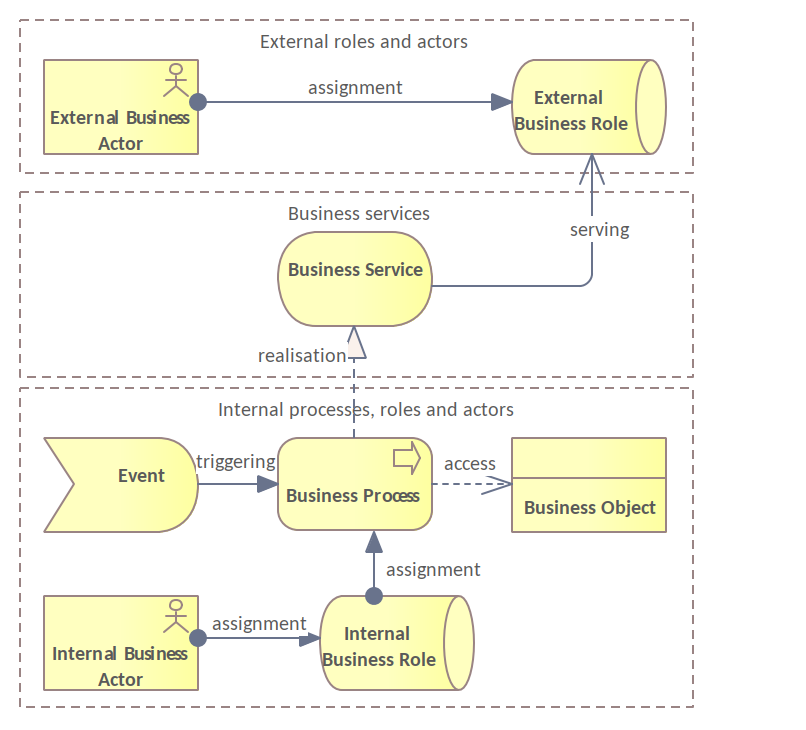
\includegraphics[width=0.4\textwidth]{images/views/Business view.png}
%		\caption{The prototypical business structure view}
%		\label{fig:business-structure-protopypical}
%	\end{wrapfigure}
	
	\begin{figure}[h]
		\centering
		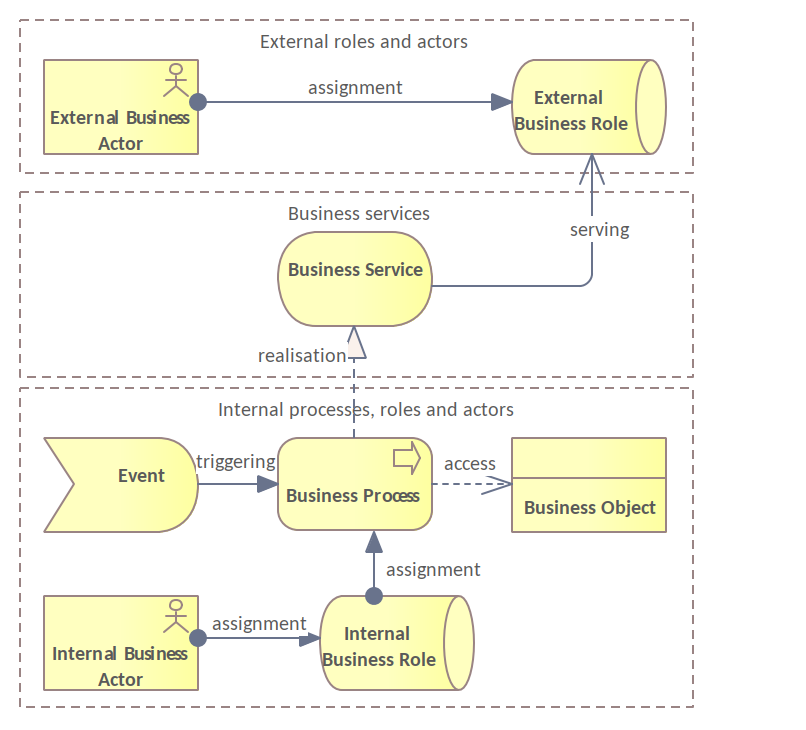
\includegraphics[width=0.4\textwidth]{images/views/Business view.png}
		\caption{The prototypical business structure view}
		\label{fig:business-structure-protopypical}
	\end{figure} 
	
	The topmost layer accounts for the external players or \textit{actors}, which represent a business entity that is capable of performing behaviour, and \textit{roles}, which represent skills and responsibilities for performing specific behaviour, and to which an actor can be assigned \citep{archimate3.1}. 
	
	The middle layer represents the \textit{services} that are offered by the organisation to the external players. A business service represents explicitly defined behaviour that a business role, business actor, or business collaboration exposes to its environment \citep{archimate3.1}.
	

	
	The lower layers accounts for the internal organisation in terms of \textit{events}, \textit{roles}, \textit{processes} and \textit{objects}. The business process represents a sequence of business behaviours that achieves a specific result such as a defined set of products or business services. The business event represents an organizational state change; while a business object represents a (passive) concept used within a particular business domain.
	

	\subsection{Current asset lifecycle stages}
	\label{sec:lifecycle-current-stages}
	
	The current asset lifecycle process is organised in six stages: \textit{inception (or evolution)}, \textit{implementation}, \textit{pre-release}, \textit{release}, \textit{publication} and \textit{consumption}. Each of the stages represents a business sub-process. Figure \ref{fig:lifecycle-current-stages} depicts the order in which stages flow and indicate that each stage process accesses a data asset, the central artefact in the diagram.
	
	\begin{figure}[h]
		\centering
		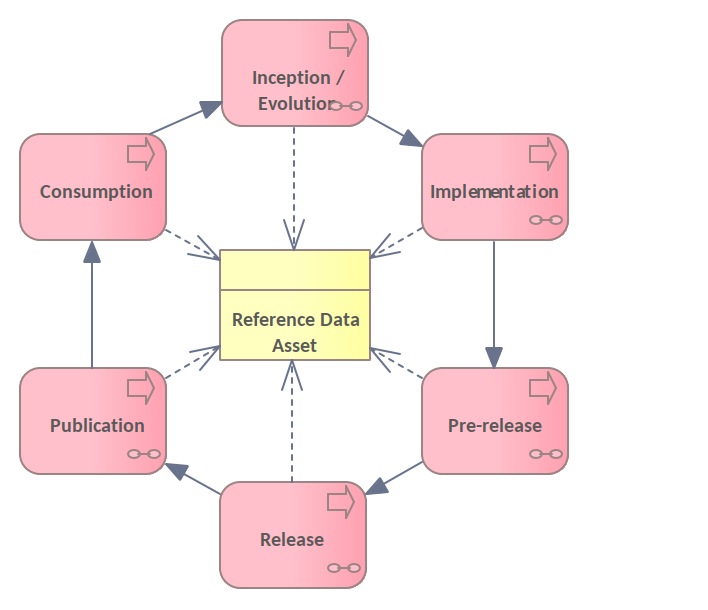
\includegraphics[width=0.5\textwidth]{images/business/Lifecycle process only (current).png}
		\caption{The current asset lifecycle stages}
		\label{fig:lifecycle-current-stages}
	\end{figure} 

	The \textit{inception} stage means that a request arrives for creating and publishing a new data asset and it is being dealt with by the team. The \textit{evolution} stage is similar only that the request is one for change of an existent data asset. There is no difference in the way these two requests are being treated and so the stage name is a conflation of the two. This stage also includes negotiating the request back with the client and then finally deciding and planning its implementation and publication. 
	
	The \textit{implementation} stage deals with actually changing, authoring, converting (Excel to XML and back) and verifying the client request. 
	
	\textit{Pre-release} marks that the content has been implemented accordingly and can be validated by a second pair of eyes implementing the \textit{four eyes principle} implemented in SU. This verification and validation is performed by checking the validation reports and by comparing the difference between the current and the previous version of the asset conveyed in a diff report. 
	
	In the \textit{release} stage the validated content is placed in a dedicated location of the common repository which indicated that the content is fit for publication. 
	
	The \textit{publication} stage deals with packaging the content and disseminating it to the selected data disseminators, Cellar being the most important one. During this stage a set of announcements and communications ensure that the main stakeholders and the broad public are aware of the published new version of the asset. 
	
	\textit{Consumption} stage is the one that happens outside the SU borders. It is the clients who use the data and then in the process come up with additional request for either changing existent assets or adding and publishing for new ones. 
	
	\subsection{Actors and roles}
	\label{sec:lifecycle-roles}	
	
	This section describes the identified actors and roles relevant to the asset lifecycle process. Figure \ref{fig:internal-roles} depicts their relations.
		
	\textit{Asset manager} (a mix of \textit{operational and business data steward}) is primarily responsible for data content, context, and associated business rules. This role is characterised by the full responsibility for the asset quality, enforcing policies and data governance processes, and ensuring asset fitness (both content and metadata) to the business needs. In the Standardisation Unit, this role is also responsible for high level interaction with the main stakeholders and important clients.
	
	\textit{Team steering committee} (also known as the team meetings) is a body composed of business, technical and analytical roles whose main purpose is to provide executive and operational guidance validating the business requests and assessing both the data management  and the broader impact, determining the implementation priority, and promoting data governance and standardisation practices.
	
%	\begin{figure}[h]
%		\centering
%		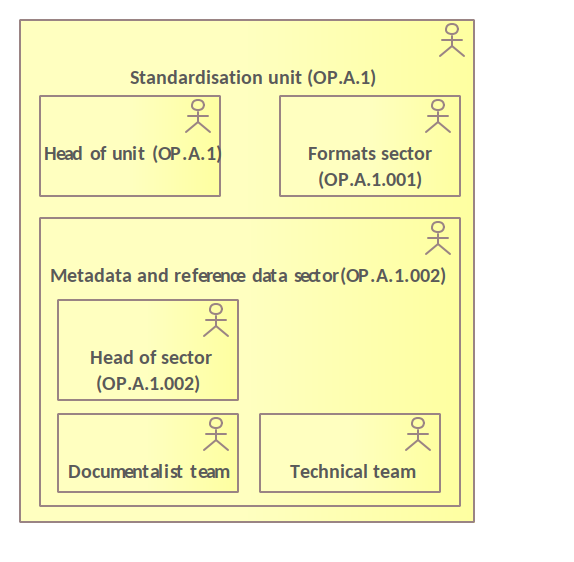
\includegraphics[width=0.47\textwidth]{images/business/Internal Business Actors.png}
%		\caption{The actors in metadata and reference data sector}
%		\label{fig:actors-team}
%	\end{figure} 
	
	\begin{figure}[h]
		\centering
		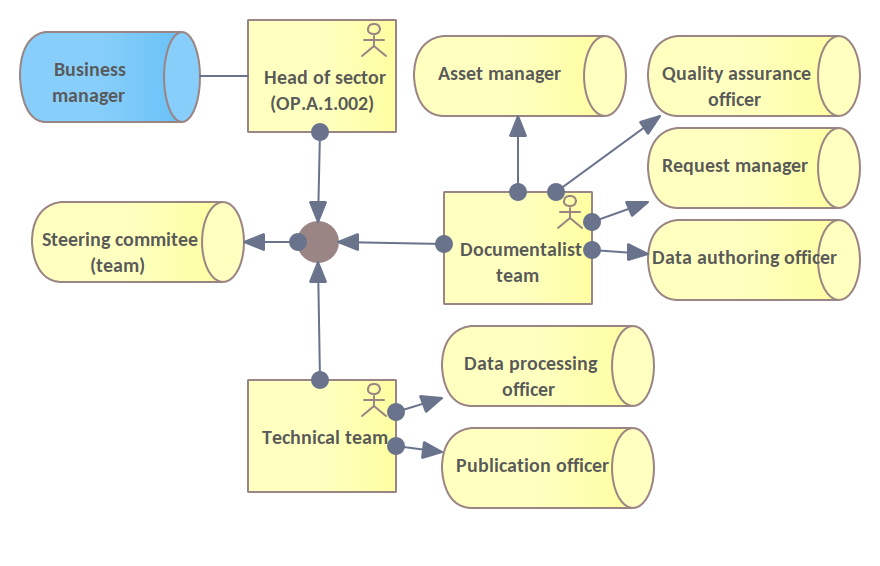
\includegraphics[width=0.7\textwidth]{images/business/Internal Roles.png}
		\caption{The internal roles in metadata and reference data sector}
		\label{fig:internal-roles}
	\end{figure}
	
	\textit{Request manager} is the interface with the client collecting the change requests, assessing the business needs and translating them into data management requirements all being summarised and documented case by case. 
	
	\textit{Data authoring officer} is responsible for editing data in a content management system implementing the cases prepared by the request manager.
	Quality assurance officers validate that the content implementation is correct from a technical and from a business point of view. 
	
	\textit{Data processing officer} is a technical role that is responsible for preparing the assets for publication. The responsibilities include but are not limited to data storage, manipulation, automatic transformation, and generation of validation and assessment reports. 
	
	\textit{Publication officer} is a technical role responsible for packaging and disseminating the assets to the specialised platforms
	
	\textit{Stakeholder steering committee} is a body representing the main clients and stakeholders ensuring data and models harmonisation, alignment of the data management practices and adoption of international standards.
	
	\textit{Client} (\textit{change requester} and \textit{data user}) is a generic external role, who on one side consumes the data and services provided by the Standardisation Unit and on the other side demands publication of new assets or modification of the existing ones. 
	
	\textit{Data disseminator} is an external role providing the Standardisation Unit with reliable data dissemination capabilities, which are meant to make the assets available for the clients.

	The external roles and stakeholders have already been addressed in the motivations structure depicted in Figure \ref{fig:stakehodlers-roles}. Each of these roles has a correspondent element in the business model and will be employed accordingly.

	\subsection{Current asset lifecycle overview}
	\label{sec:lifecycle-current}
	
	This section assembles the asset lifecycle process stages and the main internal roles together in an overview diagram depicted in Figure \ref{fig:lifecycle-current}. It indicated what roles are assigned to which processes, along with cyclical depiction of the process sequence. 
	Next we comment on the involvement of each role in the asset lifecycle process.  
	
	
	The change requester and the team steering committee are involved in the initial stage only. In this the change requester fails a new request and eventually provides additional information if it is required to do so. The team steering committee is mainly deciding which requests shall be further processed, how and when. 
	
	The asset manager is in charge of documenting, analysing and summarising the request case in the inception/evolution stage. Also it intervenes in the pre-release stage to note that the case has been implemented correctly and so that it can be closed. 
	
	Finally this role communicates with the stakeholders and broad public about the new asset changes when the asset si about to be published.
	
%	TODO: contunue
	
	\begin{figure}[h]
		\centering
		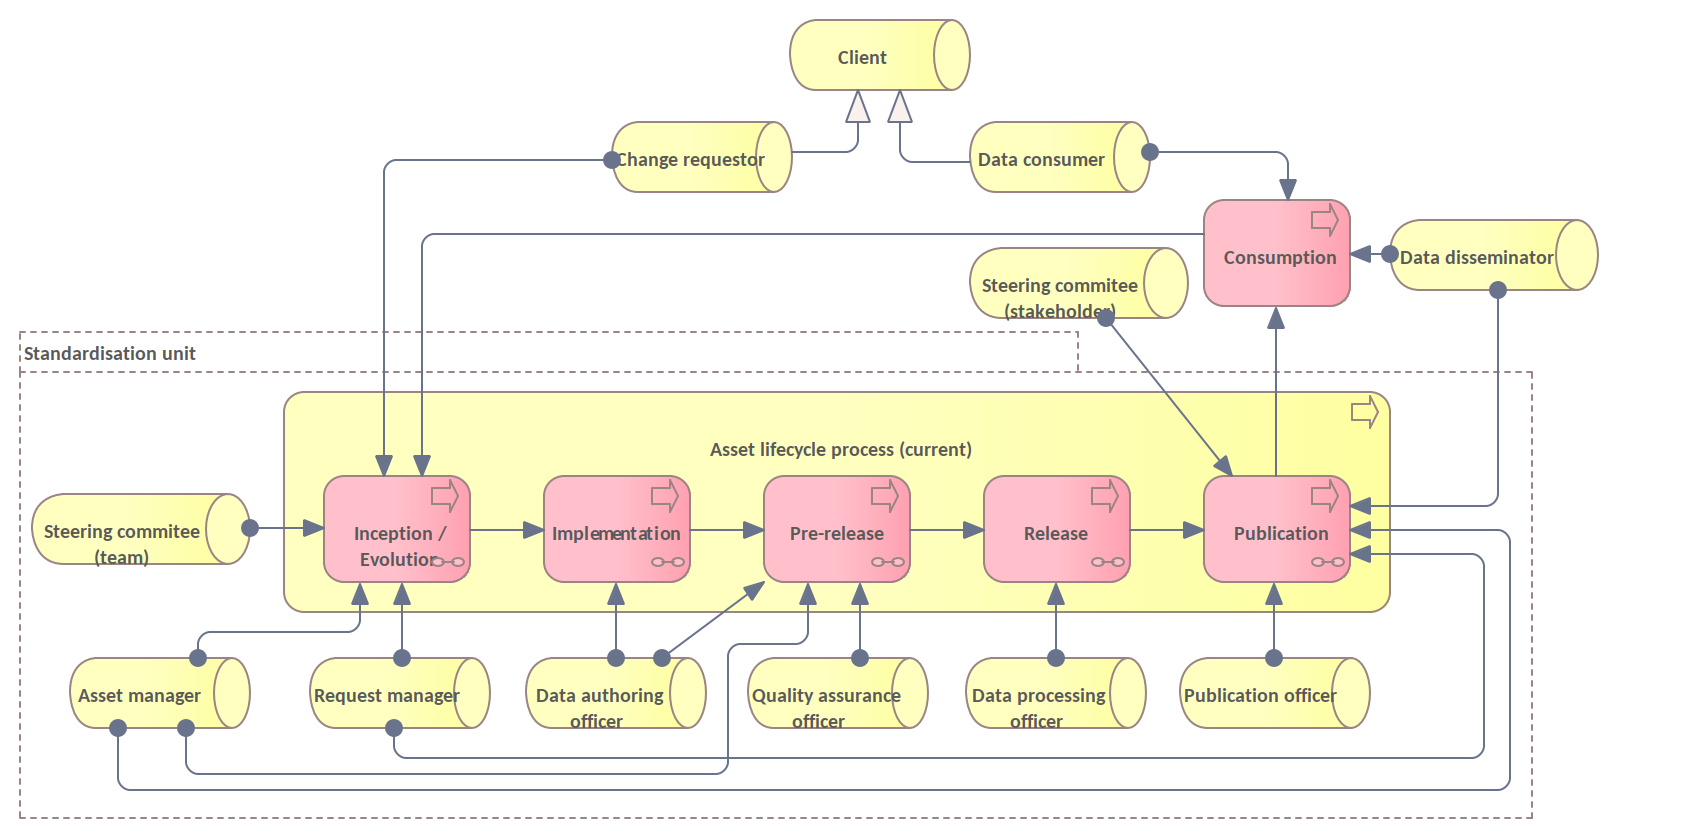
\includegraphics[width=1.05\textwidth]{images/business/Lifecycle (current).png}
		\caption{The current asset lifecycle stages and roles}
		\label{fig:lifecycle-current}
	\end{figure} 
	
	\subsection{Current inception and evolution stage}
	\label{sec:inception-current}
	
	\begin{figure}[h]
		\centering
		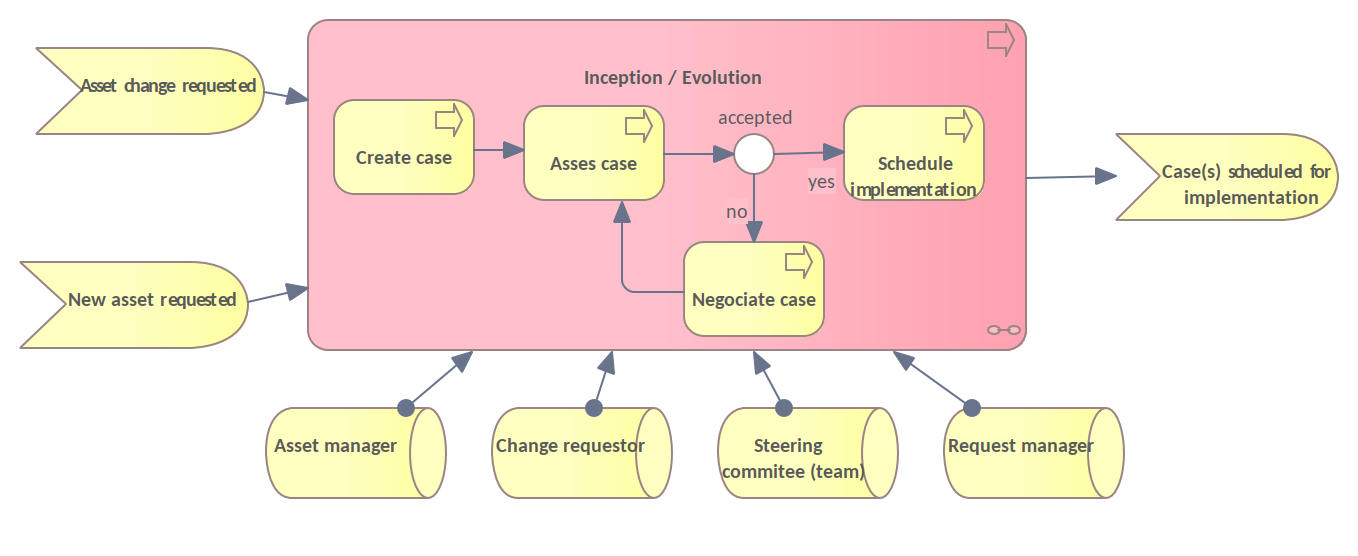
\includegraphics[width=.8\textwidth]{images/business/current/InceptionEvolution.png}
		\caption{The current process for the inception and evolution stage}
		\label{fig:evolution-current}
	\end{figure}		
	
	
	
	\subsection{Current implementation stage}
	\label{sec:implementation-current}
	
	\begin{figure}[h]
		\centering
		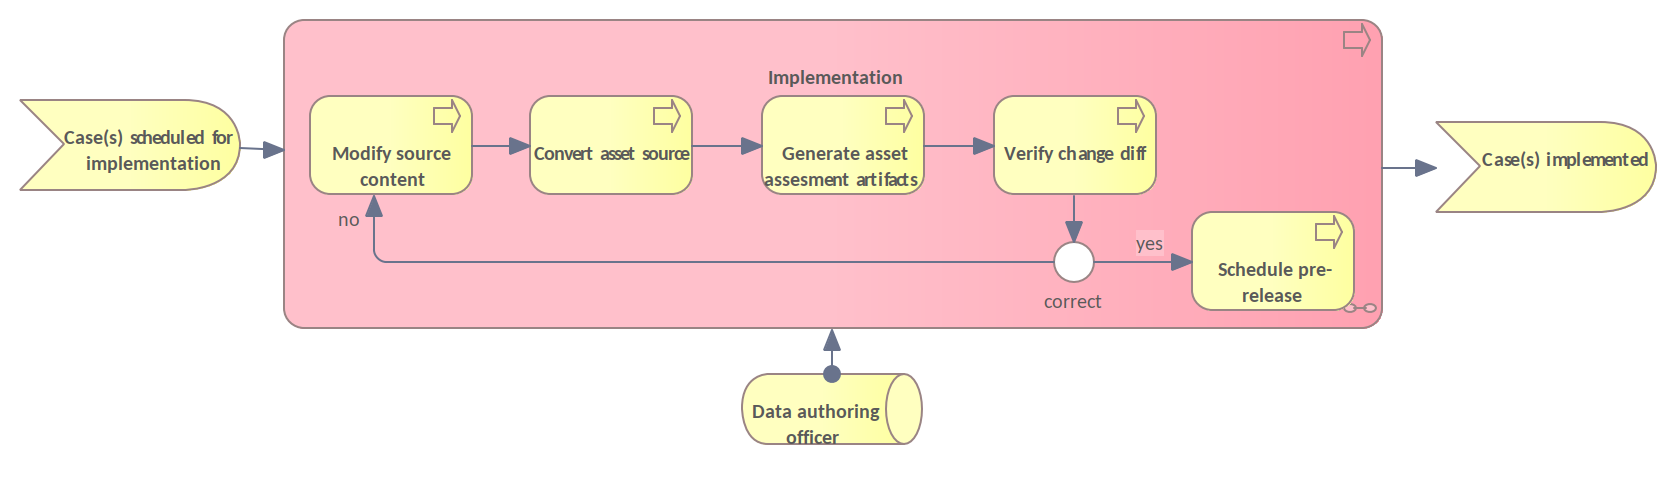
\includegraphics[width=.9\textwidth]{images/business/current/Implementation.png}
		\caption{The current process for the implementation stage}
		\label{fig:implementation-current}
	\end{figure}
	
	
	\subsection{Current pre-release stage}
	\label{sec:pre-release-current}	

	\begin{figure}[h]
		\centering
		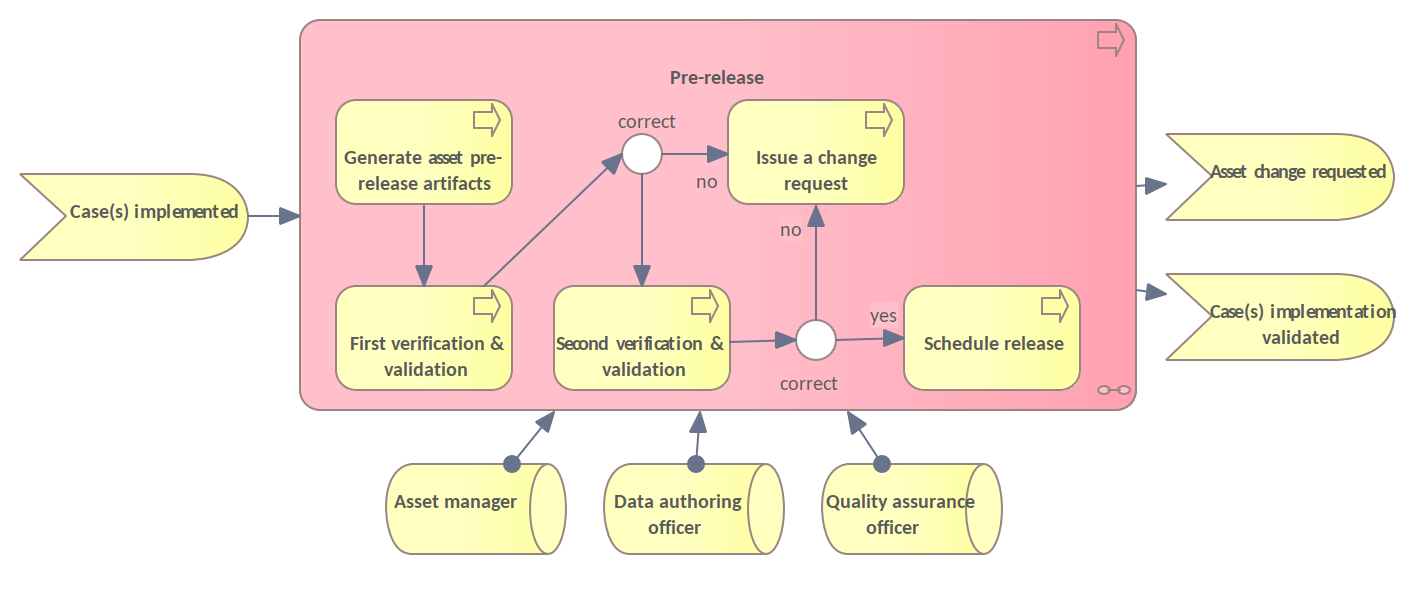
\includegraphics[width=.9\textwidth]{images/business/current/Pre-release.png}
		\caption{The current process for the pre-release stage}
		\label{fig:pre-release-current}
	\end{figure}

	\subsection{Current release stage}
	\label{sec:release-current}

	\begin{figure}[h]
		\centering
		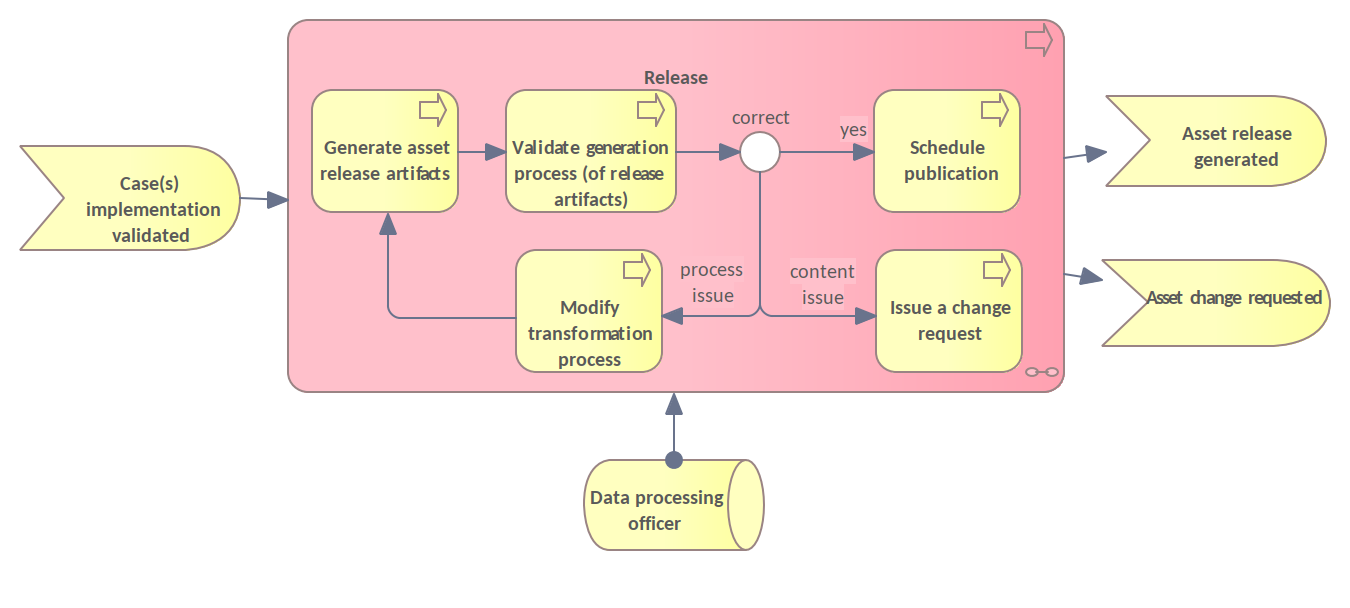
\includegraphics[width=.9\textwidth]{images/business/current/Release.png}
		\caption{The current process for the release stage}
		\label{fig:release-current}
	\end{figure}

	\subsection{Current publication stage}
	\label{sec:publication-current}
		\begin{figure}[h]
		\centering
		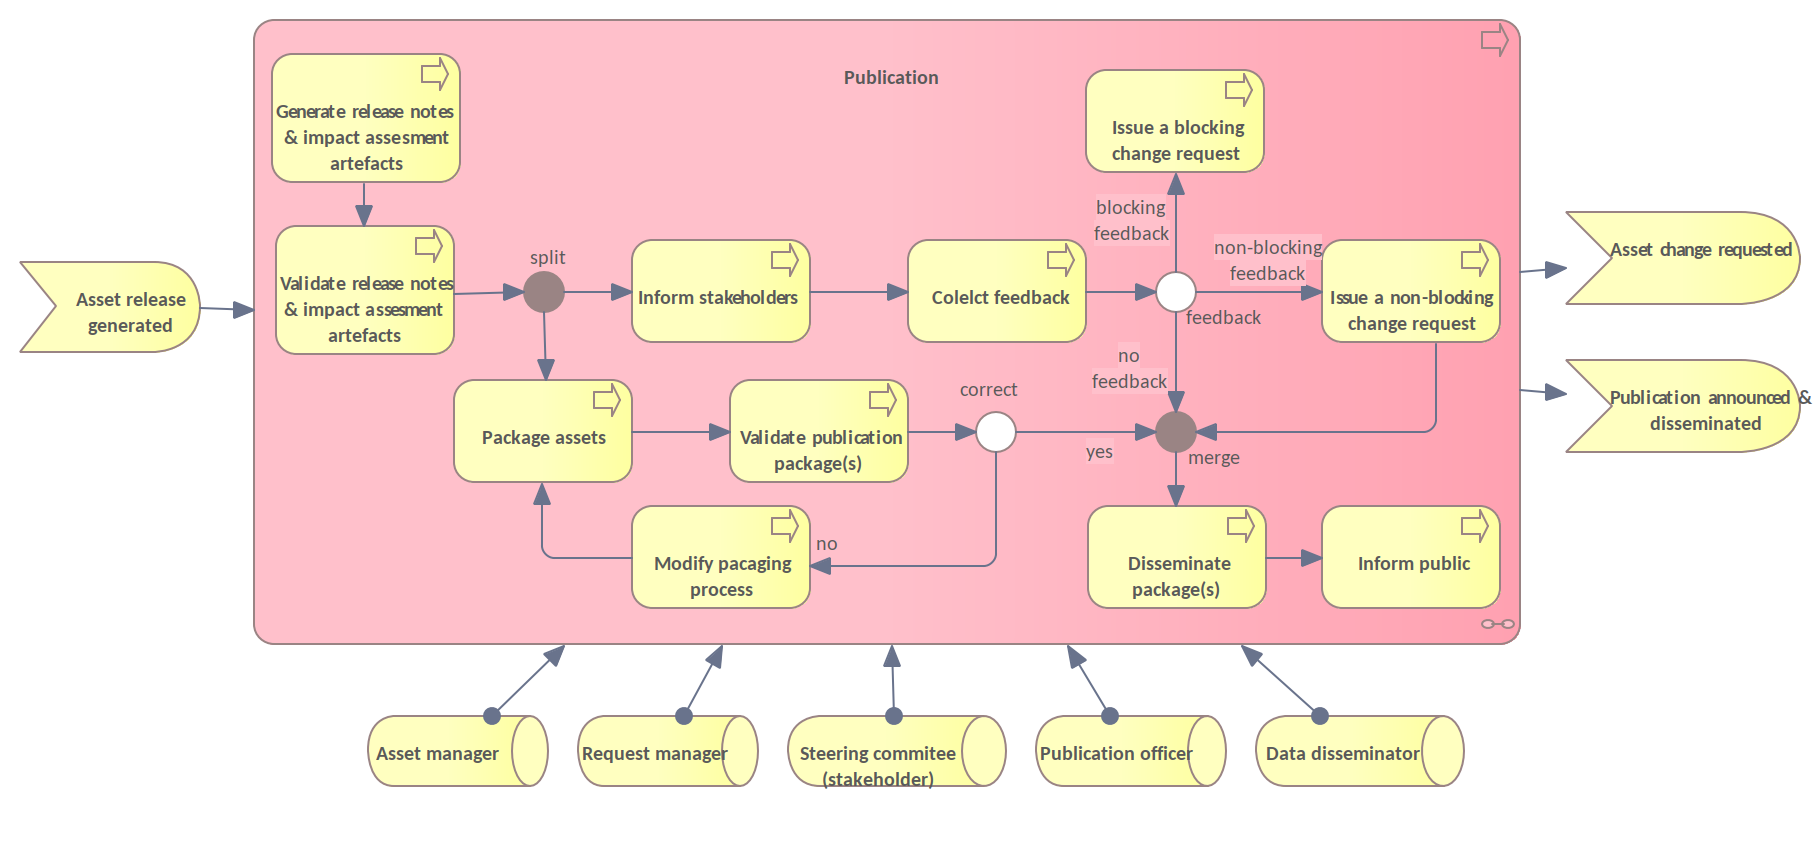
\includegraphics[width=1.01\textwidth]{images/business/current/Publication.png}
		\caption{The current process for the publication stage}
		\label{fig:publication-current}
	\end{figure}
	
	\subsection{New asset lifecycle overview}
	\label{sec:lifecycle-new}
	
	\begin{figure}[h]
		\centering
		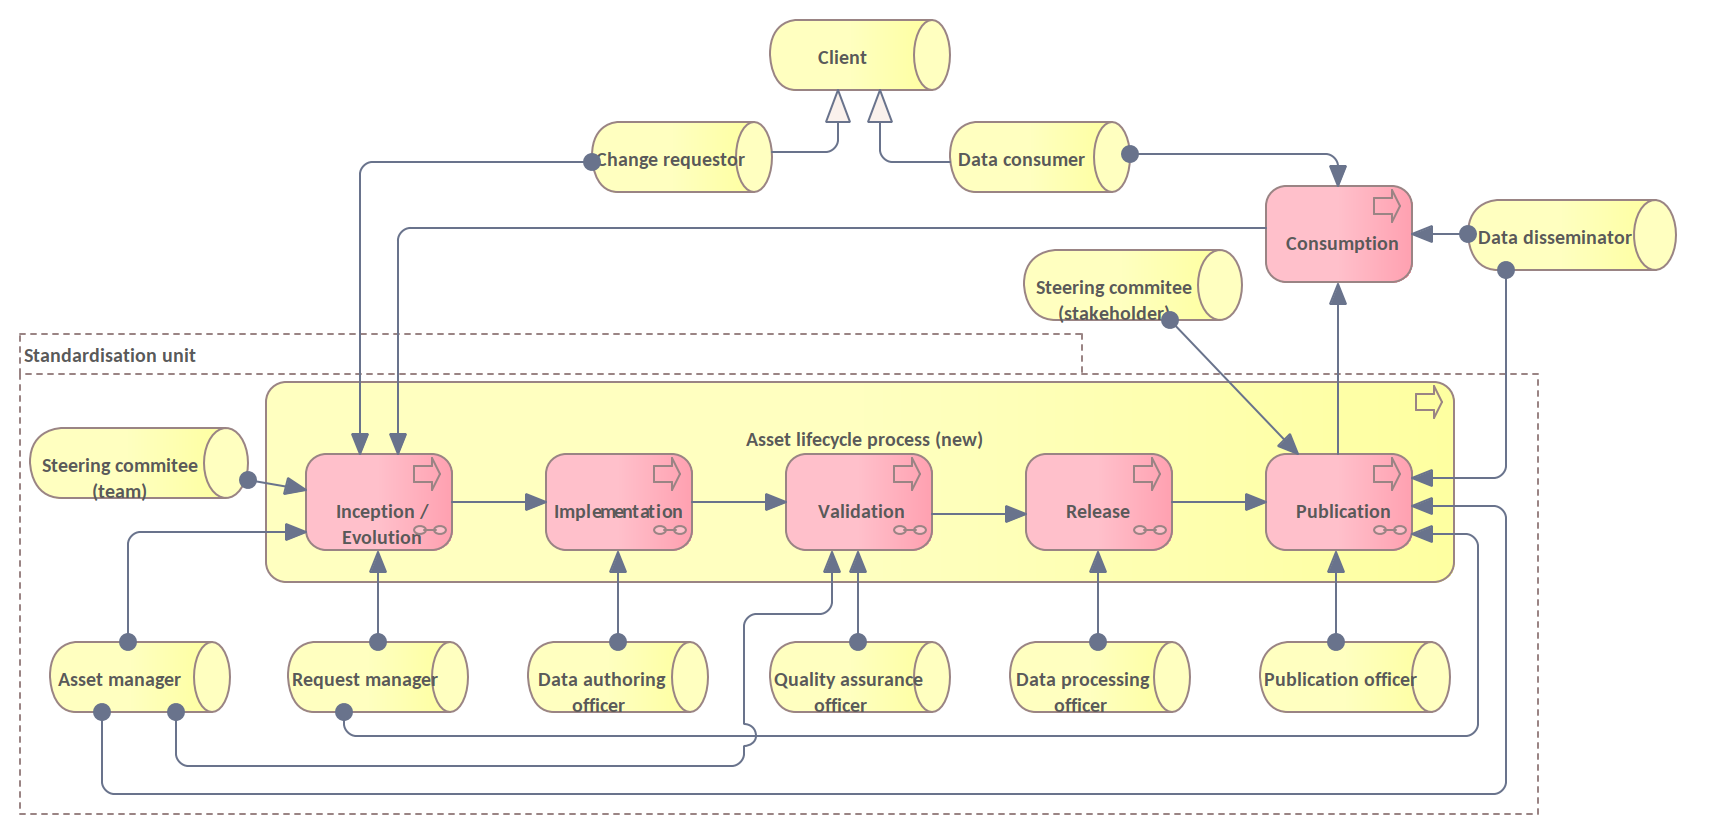
\includegraphics[width=1.05\textwidth]{images/business/Lifecycle (new).png}
		\caption{The current asset lifecycle stages and roles}
		\label{fig:lifecycle-new}
	\end{figure} 	

	\subsection{New implementation stage}
	\label{sec:implementation-new}

	\begin{figure}[h]
		\centering
		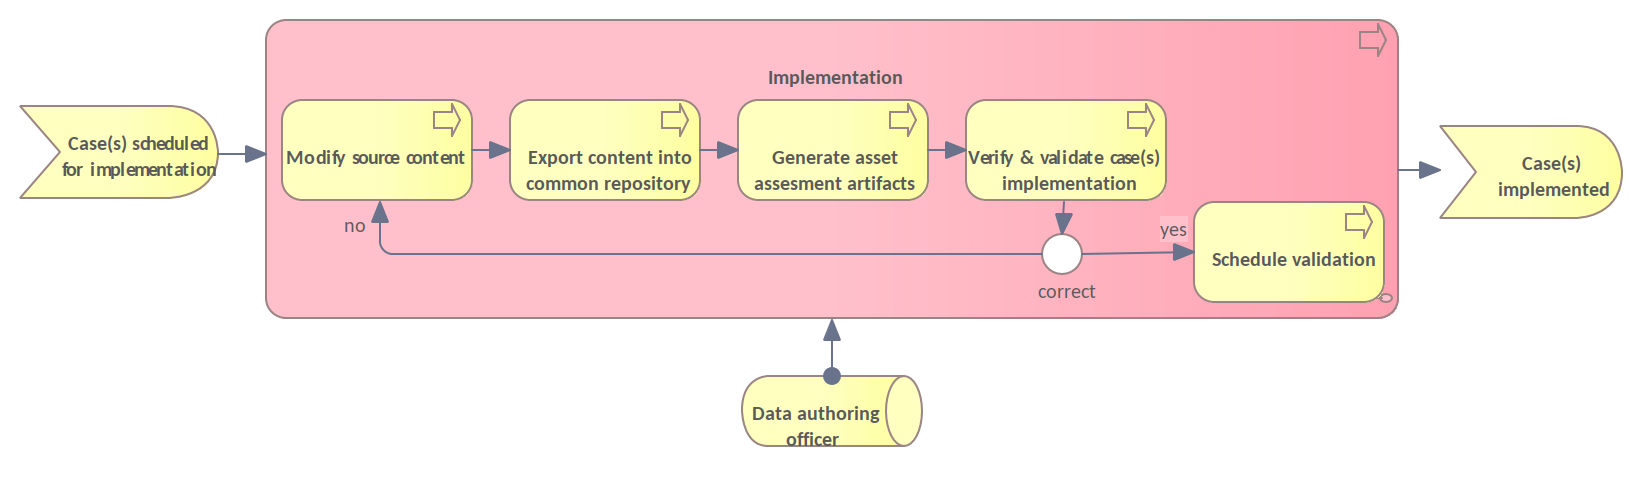
\includegraphics[width=1.05\textwidth]{images/business/new/Implementation.png}
		\caption{The new process for the implementation stage}
		\label{fig:implementation-new}
	\end{figure} 		
	
	\subsection{New validation stage}
	\label{sec:validation-new}	

	\begin{figure}[h]
		\centering
		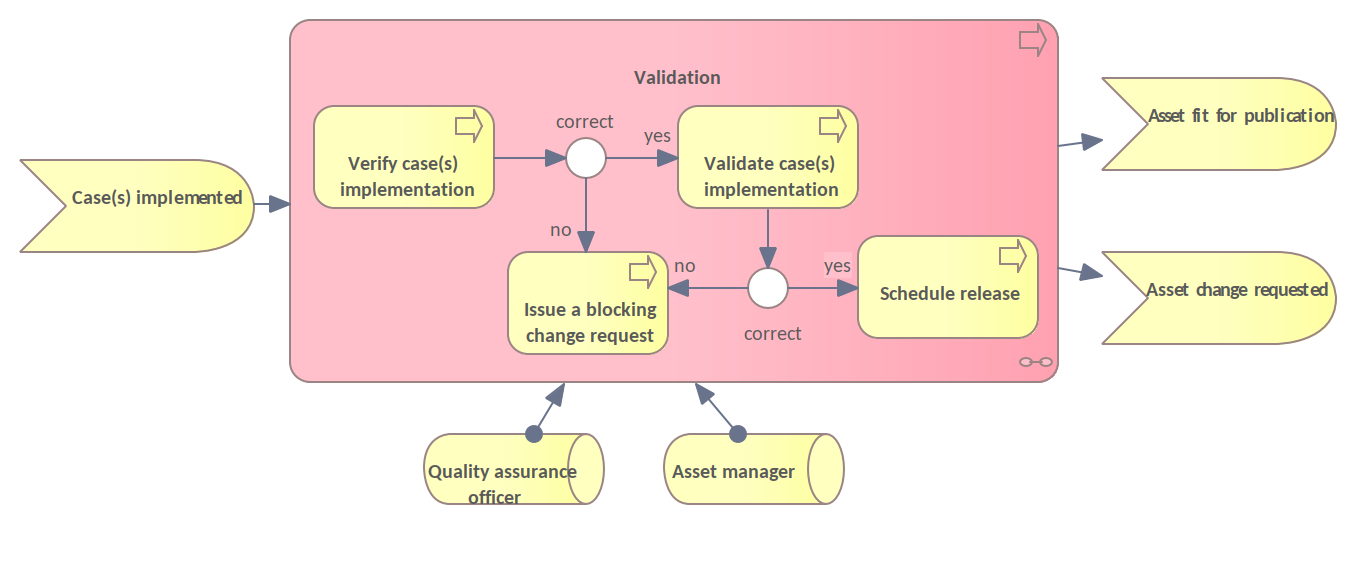
\includegraphics[width=.9\textwidth]{images/business/new/Validation.png}
		\caption{The new process for the validation stage}
		\label{fig:validation-new}
	\end{figure} 		
	
	\subsection{New release stage}
	\label{sec:release-new}
	
	\begin{figure}[h]
		\centering
		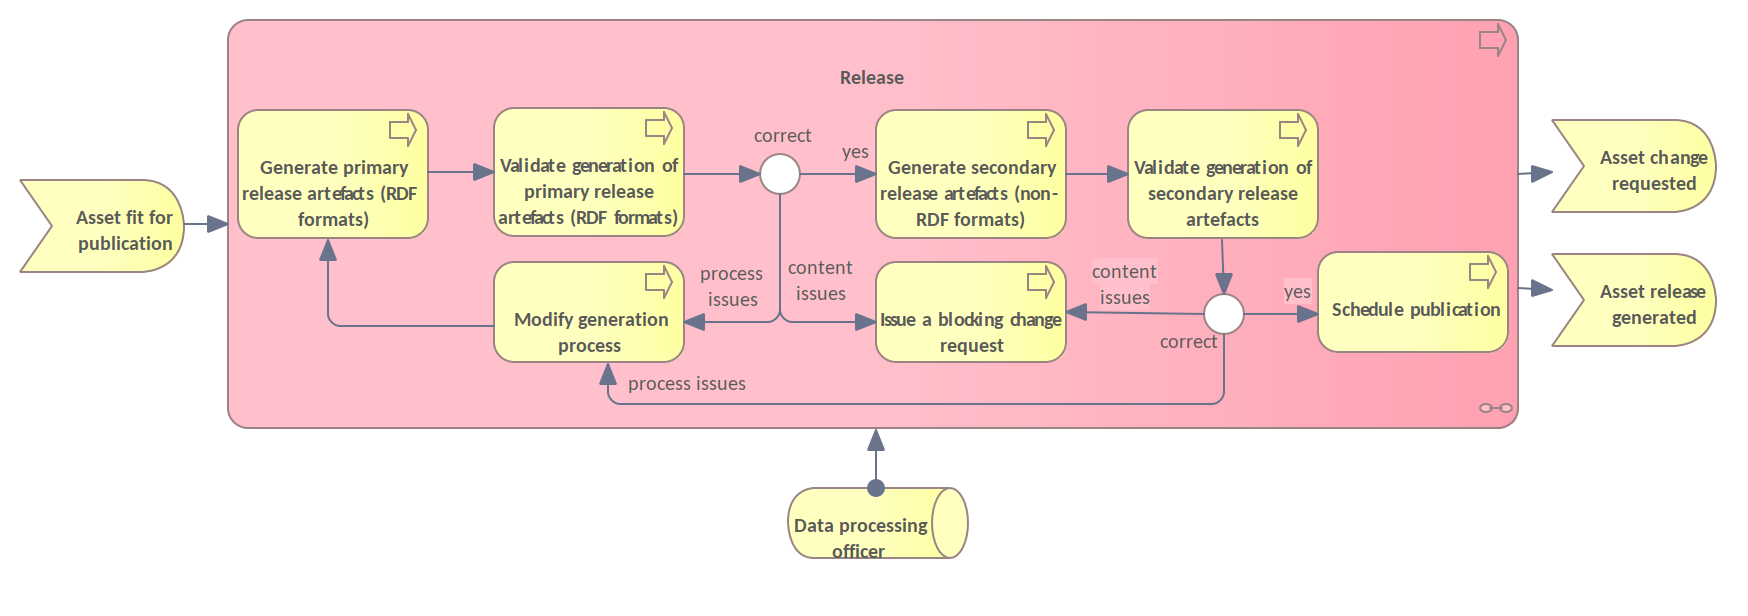
\includegraphics[width=1.05\textwidth]{images/business/new/Release.png}
		\caption{The new process for the release stage}
		\label{fig:release-new}
	\end{figure}